\documentclass{article}

\title{Modelo de Processo}
\usepackage[utf8]{inputenc}
\usepackage{float}
\usepackage{graphicx}										
\usepackage[brazil]{babel}								
\usepackage[ddmmyyyy]{datetime}
\usepackage{color}
\usepackage[svgnames]{xcolor}
\usepackage{sectsty}
\allsectionsfont{\usefont{OT1}{phv}{b}{n}}

\sectionfont{\usefont{OT1}{phv}{b}{n}}

\usepackage{fancyhdr}	
	\pagestyle{fancy}	
\usepackage{lastpage}

\lhead{}
\chead{}
\rhead{}

\lfoot{\footnotesize \texttt Processo de Gerencia de Configurações}

\cfoot{}
\rfoot{\footnotesize página \thepage\ de \pageref{LastPage}}	% "Page 1 of 2"
\renewcommand{\headrulewidth}{0.0pt}
\renewcommand{\footrulewidth}{0.4pt}

\usepackage{lettrine}
\newcommand{\initial}[1]{%
\lettrine[lines=3,lhang=0.3,nindent=0em]{
\color{DarkGoldenrod}
{\textsf{#1}}}{}}

\usepackage{titling}

\newcommand{\HorRule}{\color{DarkGoldenrod}%			% Creating a horizontal rule
\rule{\linewidth}{1pt}%
}

\pretitle{\vspace{-30pt} \begin{flushleft} \HorRule 
\fontsize{50}{50} \usefont{OT1}{phv}{b}{n} \color{DarkRed} \selectfont 
}

\title{Processo de Gerência de Configurações}				



\posttitle{\par\end{flushleft}\vskip 0.5em}

\preauthor{\begin{flushleft}
\large \lineskip 0.5em \usefont{OT1}{phv}{b}{sl} \color{DarkRed}}
\author{Alexandre L'Erario, Fulano de Tal }  	% Author name goes here


\postauthor{\footnotesize \usefont{OT1}{phv}{m}{sl} \color{Black} 
\\Universidade Tecnológica Federal do Paraná - Câmpus Cornélio Procópio 								% Institution of author
\par\end{flushleft}\HorRule}

\date{}																
\title{Processo de Gerencia de Configurações}
\author{Lucas Joaquim, Josiel Faleiros e Rafael Santos } 

\begin{document}
	\maketitle
	\pagenumbering{arabic}
	\newpage
	\tableofcontents
	\newpage
	\section{Introdução}
    Nesse documento foi especificado um processo de gerencia de configuração para a empresa Software Supimpa Tecnologia (2ST). Usando como base as normas da CMMI-DEV. A empresa possui o produto de software Klassic e conta com 10 desenvolvedores.
    \section{Baselines}
	    Nessa seção serão definidos identificados os itens de configuração e as baselines presentes no projeto que serão versionados e controlados.
	    \subsection{Identificando Items de Configuração}
          Na seguinte tabela constam os itens de configuração e seus respectivos identificadores.
	  	\begin{table}[H]
			\begin{tabular}{l c r}
                  \textbf{Item} & \textbf{Identificador}\\
                  \hline
                  Diagrama de Caso de Uso & UC \\
                  Diagrama de Classe & CD \\
                  Diagrama de Sequência  & SD \\
                  Diagrama de Pacotes  & PD \\
                  Planilha clientes software & PCS\\
                  Código fonte  & CF\\
                  Documento LaTeX & TEX \\
              \end{tabular}\\
              \caption{Itens sob controle}
          \end{table}
          \subsection{Baselines do projeto}
          \begin{table}[H]
              \begin{tabular}{l l l}
                  \textbf{Baseline} & \textbf{Itens relacionados} & \textbf{status}\\
                  \hline
                  Plano de Gerência de Configuração & TEX & em desenvolvimento \\
                  Documentação & CD, SD, UC, PD, PCS & em desenvolvimento \\
                  Produto & Código fonte & em desenvolvimento\\
              \end{tabular}\\
              \caption{Baseline}
          \end{table}
    \section{Controle de Mudanças}
    	\subsection{Ferramentas}
        No ciclo de desenvolvimento do projeto serão utilizadas as seguintes ferramentas para a criação e versionamento dos artefatos, bem como meios para realização de auditoria.
        \begin{itemize}
          \item Git - é um sistema de controle de versão distribuído e um sistema de gerenciamento de código fonte, com ênfase em velocidade. 
          \item Github - é uma plataforma de hospedagem de código-fonte com controle de versão usando o Git.
          \item Astah - é um software para modelagem uml. 
          \item Bpmn.io - é um software para diagramação online.
        \end{itemize}
         \subsection{Repositórios}
         Abaixo constam os repositórios do projeto:
	         \begin{itemize}
		         \item Documentation - Contém toda a documentação do projeto. https://github.com/ProdutoInova/Documentation.git.
		         \item ProdutoInova - Contém todo o código do projeto. https://github.com/ProdutoInova/Inova.git.
		         \item modulo-cidade - Contém a implementação do módulo cidade. https://github.com/ProdutoInova/modulo-cidade.git.
		      \end{itemize}
        \subsection{Políticas de versionamento}
        Será usado o seguinte formato para versionamento: 0.0.0. Para o incremento dos números deverão ser seguidas as seguintes políticas:
        \begin{itemize}
        	\item O número mais a esquerda é incrementado quando são realizadas uma ou mais mudanças que resultam na perda de compatibilidade com a versão anterior.
			\item O número do centro é incrementado quando é adicionada uma ou mais funcionalidades, mas mantendo a compatibilidade com a versão anterior. 
			\item O número mais a direita é incrementado quando é realizada correções de bugs, também mantendo a compatibilidade com a versão anterior. 
		\end{itemize}
		\subsection{Auditoria}
			Será utilizado o audit log do Github para avaliação das ações realizadas pelos membros do projeto. O audit log inclui detalhes como quem executou a ação, qual foi a ação e quando foi realizada.
			\newline
			É possível realizar as seguintes ações:
			\begin{itemize}
				\item Em que repositório uma ação foi realizada.
				\item O usuário que realizou a ação.
				\item A ação que foi realizada.
				\item Em que país a ação teve lugar.
				\item A data e hora em que a ação ocorreu.
			\end{itemize}
        \subsection{Processo para adesão de novos desenvolvedores}
	        \begin{figure}[H]
	        	\centering
	        	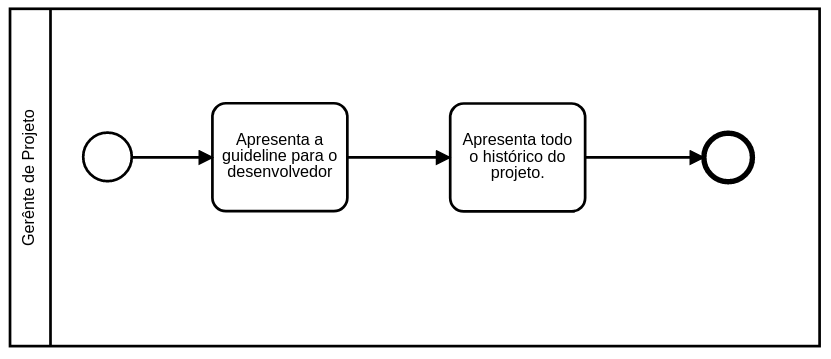
\includegraphics[width=0.7\linewidth]{processo_adesao_novo_desenvolvedor}
	        	\caption{}
	        	\label{fig:processoadesaonovodesenvolvedor}
	        \end{figure}
	        
        \subsection{Processo para adicionar novas funcionalidades}
			\begin{figure}[H]
				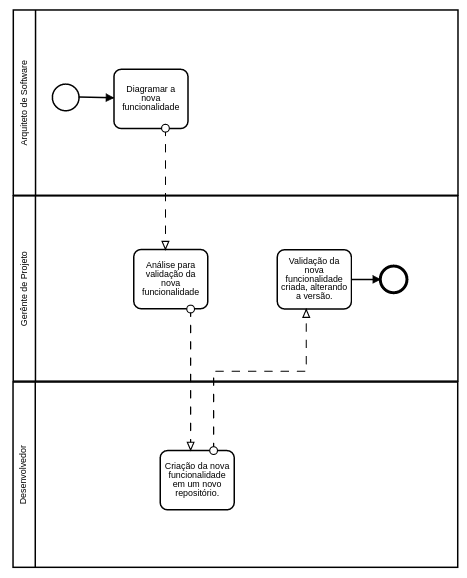
\includegraphics[width=\linewidth]{processo_nova_funcionalidade}
				\caption{Adição de novas funcionalidades.}
				\label{fig:processonovafuncionalidade}
			\end{figure}
        \subsection{Processo para fazer atualizações}
			\begin{figure}[H]
				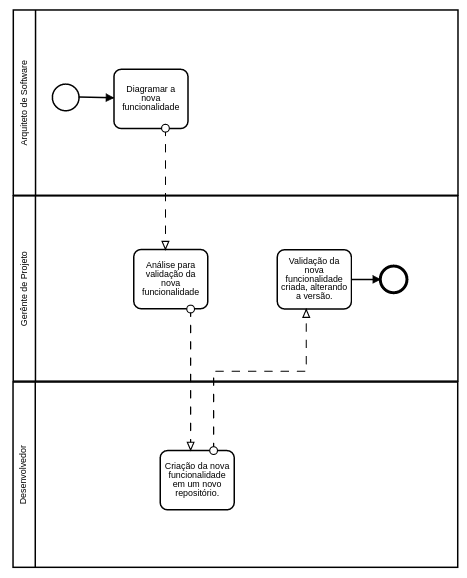
\includegraphics[width=\linewidth]{processo_nova_funcionalidade}
				\caption{Fazer atualizações.}
				\label{fig:processonovafuncionalidade}
			\end{figure}
        \subsection{Processo para correção de bugs}
	        \begin{figure}[H]
	        	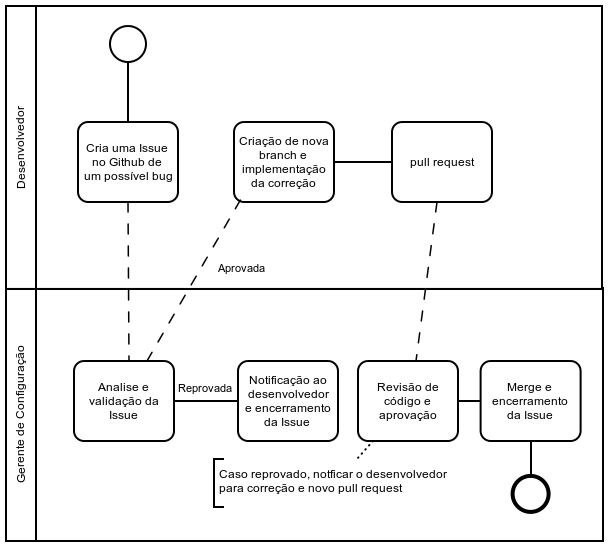
\includegraphics[width=\linewidth]{bug.png}
	        	\caption{Correção de bugs.}
	        \end{figure}
        \subsection{Processo para criação de distribuições}
			\begin{figure}[H]
				\centering
				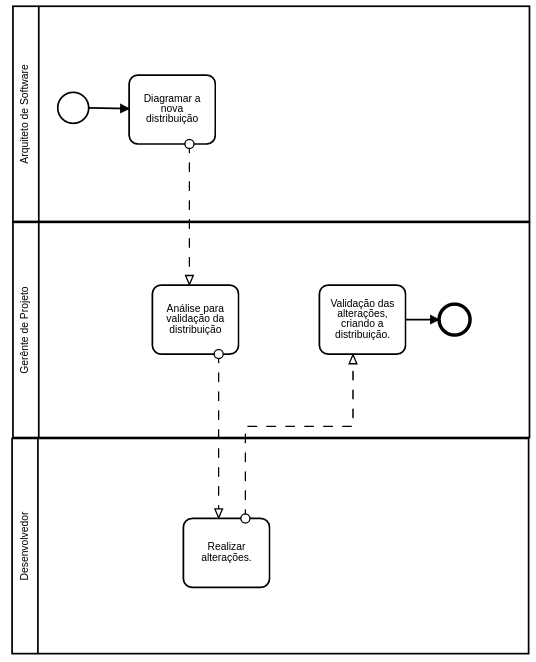
\includegraphics[width=0.7\linewidth]{processo_criacao_distribuicao}
				\caption{}
				\label{fig:processocriacaodistribuicao}
			\end{figure}

    \section{Controle dos clientes}
    Cada cliente pode possuir funcionalidades diferentes, tendo então uma tabela para controle de quais clientes possuem quais funcionalidades e suas versões.
        \begin{figure}[H]
			\centering
			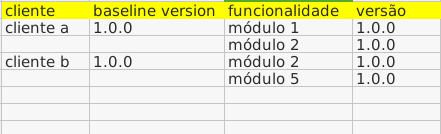
\includegraphics[width=0.7\linewidth]{controle_cliente_software.png}
			\caption{}
			\label{fig:controleclientesoftware}
		\end{figure}
        
    \newpage
	\begin{appendix}
		\listoffigures
		\listoftables
	\end{appendix}
\end{document}
